\chapter{Mechanical Design}

\graphicspath{{./Figures/Mechanical Design/}}



	
%	\item Outline the purpose and scope of the chapter.

 Modeling In this chapter, the details of the mechanical design are presented. where it goes from the initial conceptual design to the final design showing in the process the design decision-making for each critical point, This chapter emphasis the detailed description of the precise placement and alignment of different components such as the motors, wheels, battery, boards, and others to maintain the seamless integration of all the components into the robot body.
%	\item Briefly describe the mechanical design's role in the overall project.
\newline
The mechanical design serves as an important pillar to define the new physical form, size, and shape of the TWIPR. Depending on how these criteria are defined, the robot would interact with the environment. taking into account that the design directly influences the center of gravity, which is crucial to consider in our robot due to the inverted pendulum nature to be able to balance and maintain the upright position. In addition to the impact that the design has on the maneuverability of the robot and how it would respond to the control signals to be able to execute a task.

\newpage


\section{Design Objectives and Requirements}

%	Detail the primary objectives of the mechanical design
	The main objective is to come up with a new design for a multiple joints Robot to perform complex dynamic movements. this robot would be based on the Two wheeled inverted pendulum robot. The new design would add more degrees of freedom to enable the more complex movements.This enhances the robot capabilities where it can execute more diverse scenarios. 
%	\item List the requirements that the design must meet (e.g., weight limits, size constraints, mobility requirements).
	Initially, the main requirement was to add more two degrees of freedom where originally it used to have one degree of freedom in the wheels. The new design has three degrees of freedom one in the wheels, one as a knee joint and one as a hip joint. The current design has two identical legs.

\section{Conceptual Design}
%Discuss the initial design concepts.
As for the initial design concepts the body was that main point of focus as shown in the figure.Three initial designs where considered mainly for the body.\ Symmetrical vertical body in figure A, symmetrical horizontal body in figure B and leaning forward body in figure C.
\ For the three designs, two independent legs where considered.
two designs where considered for the legs, the normal joint leg and the compliant leg
% figure of the initial design concepts
\begin{figure}[h]
	\centering
	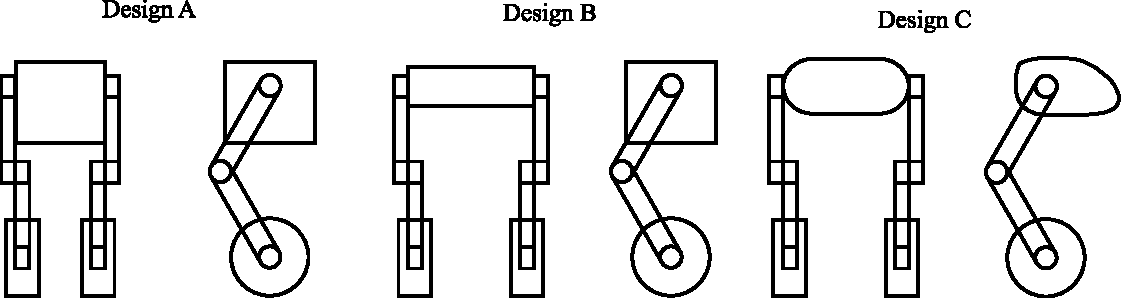
\includegraphics[width=1\linewidth]{Conceptual Design}
	%\includegraphics[width=0.5\linewidth]{Figures/Mechanical Design/Conceptual_Design}
	\caption{Initial Design Concepts}
	\label{fig:initialdesigns}
\end{figure}

the compliant leg is more flexible and can be used to absorb the shock from the ground.\ The normal joint leg is more rigid and can be used to generate more torque.in addition, the normal is more relative to our use-case as it can precisely control the position of the leg.
% figure for the leg designs
\begin{figure}[h]
	\centering
	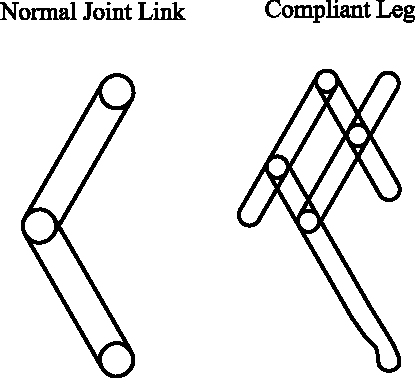
\includegraphics[width=0.4\linewidth]{Leg Design}
	%\includegraphics[width=0.5\linewidth]{Figures/Mechanical Design/Conceptual_Design}
	\caption{Leg Designs}
	\label{fig:legdesigns}
\end{figure}




%Explain the decision-making process for selecting the final concept.
% Include sketches or early design models.

\section{Detailed Design Development}
\begin{itemize}
	\item Elaborate on the development of the detailed mechanical design.
	\item Discuss material selection and the rationale behind these choices.
	\item Include detailed CAD drawings and design schematics.
\end{itemize}
\section{Design for Manufacturability and Assembly}
\begin{itemize}
	\item Discuss how the design facilitates manufacturing and assembly..
	\item Explain any design choices made to simplify these processes of manufacturing and assembly.
\end{itemize}
\section{Prototyping and Iterative Design}
\begin{itemize}
	\item Discuss the process of prototyping.
	\item Explain how feedback from prototyping phases was incorporated into design revisions.
\end{itemize}

